
\lecture{3}{Energy in Thermal Physics}{Qiang Zhu}{scribe-name1,2,3}
%\footnotetext{These notes are partially based on those of Nigel Mansell.}
% **** YOUR NOTES GO HERE:
% Some general latex examples and examples making use of the
% macros follow.  
%**** IN GENERAL, BE BRIEF. LONG SCRIBE NOTES, NO MATTER HOW WELL WRITTEN,
%**** ARE NEVER READ BY ANYBODY.

\section{Some useful equations} % Don't be this informal in your notes!
\begin{equation} \label{idealgas} PV = nRT = NkT \end{equation}
\begin{equation} \label{Avogadro} N = n \times N_A \end{equation}
\begin{equation} \label{PV-micro} PV = Nm{\overline v_x^2} = NkT \end{equation}
\begin{equation} \label{eqpartition} U_\text{thermal} = N \cdot f \cdot \frac{1}{2}kT \end{equation}

How to count the number of degree of freedom ($f$)
\begin{enumerate}
\item{translation, rotation, vibration as a function of temperature}
\item{number of atoms in the molecule, monoatomic, diatomic, .etc}
\item{internal symmetry}
\end{enumerate}

\section{First law of thermodynamics}
By conservation of energy, the change in total thermal energy is the sum of heat entered the system and work done on the system,
\begin{equation} \label{1st} \Delta{U} = Q + W \end{equation}
Q: heat transfer by conduction, convection, radiation.\\
W: mechanical/electric/chemical work. \\

\section{Compression Work and $PV$ diagram}
while we already know how to calculate U according to eq \ref{eqpartition}, let's try to figure out how to calculate W.
We always start from its original definition,
\begin{equation} \label{work1} \Delta W = F \Delta{X} \end{equation}
Suppose this is a quasistatic compression, i.e, every step is very slow and reversible, then we have
\begin{equation} \label{work2} \Delta W = P A \Delta{X} \end{equation}
for each step. By merging $A\Delta{X}$ term, we get
\begin{equation} \label{work3} \Delta W = - P \Delta{V} \end{equation}

A simple way to check if the derived equation is correct. W and -$P\Delta{V}$ both have the unit of J.\\
How to calculate -$P\Delta{V}$?
\begin{enumerate}
\item{$P$ is fixed during compression}
\item{$P$ is not constant}
\end{enumerate}
We need to integrate each small step for eq.\ref{work3}, hence we have
\begin{equation} \label{work4} W = -\int_{V_{i}}^{V_{f}} P(V)dV. \end{equation}
Graphically, it means the total area under the graph of P v.s. V. \\

%\begin{figure}[h]
%\centering
\begin{tikzpicture}[thick]
\draw [->](0,0) -- (0,4);
\draw [->](3,2) -- (1,2); 
\draw [->](0,0) -- (4,0);
\node at (2,-0.5) {$V$};
\node at (-0.5,2) {$P$};
\draw [->](10,0) -- (10,4);
\draw [->](13,3) -- (11,2); 
\draw [->](10,0) -- (14,0);
\node at (12,-0.5) {$V$};
\node at (9.5,2) {$P$};

\end{tikzpicture}
%\end{figure}


{\bf Exercises}\\
(Problem 1.32):\\
By applying a pressure of 200 atm, you can compress water to 99\% of its usual volume. Sketch the process on a PV diagram, and estimate the work required to achieve it. Does the result surprise you? \\\\\\\\\\\\\\


(Problem 1.33):
Analyze the cyclic process shown as follows,\\\\

\begin{tabular}{|c | c | c | c | c |}
\hline
    & A & B & C & Total \\\hline
$W$ &   &   &   &\\\hline
$Q$ &   &   &   &\\\hline
$U$ &   &   &   &\\\hline
\end{tabular}\\\\


\subsection{Compression on ideal gas}
Let's think about how compression is done on the ideal gas. There are two extremes as follows.
\begin{enumerate}
\item{very slow that the temperature doesn't change at all, i.e., isothermal compression}
\item{very fast that the no heat escapes from the gas, i.e., adiabatic compression}
\end{enumerate}
What do they indicate:
\begin{enumerate}
\item{if $T$ doesn't change, $U$ is constant.}
\item{if no heat escapes, $Q$ is zero.}
\end{enumerate}

\subsection{Isothermal Compression}
Under isothermal condition,
\begin{equation} \label{isot} 
 W = -\int_{V_{i}}^{V_{f}} P(V)dV = -NkT \int_{V_{i}}^{V_{f}} \frac{1}{V}dV.
\end{equation}
Remember some special functions, $e^x$, ln$x$, sin($x$), cos($x$).
\begin{equation} \label{isot} 
 W = -NkT(\textrm{ln}V_f - \textrm{ln}V_i)
\end{equation}

Since $U$ is constant, $Q$ is simply -$W$.


\subsection{Adiabatic Compression}
Remember $U$=$W$ under adiabatic condition, hence we have 
\begin{equation} \label{du} dU = \frac{f}{2}NkdT, \end{equation}
\begin{equation} \label{dW} dW = -PdV. \end{equation}
Since $dU$=$dW$
\begin{equation} \label{duw1} -PdV = \frac{f}{2}NkdT. \end{equation}
By plugging in $PV = NKT$, we get
\begin{equation} \label{duw2} -\frac{dV}{V} = \frac{f}{2} \frac{dT}{T}. \end{equation}
Let do integrate here,
\begin{equation} \label{duw3} \int_{V_{i}}^{V_{f}}  -\frac{dV}{V} = \frac{f}{2} \int_{T_{i}}^{T_{f}} \frac{dT}{T}. \end{equation}
then we get
\begin{equation} \label{duw4} \textrm{ln}\frac{V_f}{V_i} = \frac{f}{2} \textrm{ln}\frac{T_i}{T_f}. \end{equation}
To remove the logarithmic sign, we have 
\begin{equation} \label{duw5} V_fT_f^{f/2} = V_iT_i^{f/2} = \textrm{const}. \end{equation}
Alternatively, we can also rewrite it in the form of $P$ instead of $T$,
\begin{equation} \label{duw6} V^{\gamma}P = \textrm{const}. \end{equation}
where ${\gamma}$ = $\frac{f+2}{f}$ is called adiabatic exponent.\\
Homework: how to prove it? It will be intensively used in the following class!

%\begin{figure}[h]
%\centering
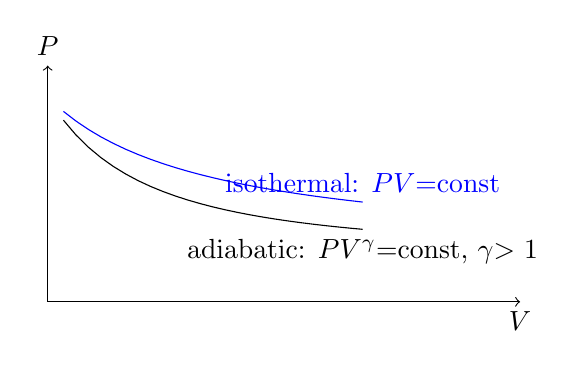
\begin{tikzpicture}[x=2cm, y=2cm]
\draw [->] (1,-0.3) -- (4, -0.3) node[below]{$V$};
\draw [->] (1,-0.3) -- (1, 1.2)  node[above]{$P$};
\draw [color=blue, domain=1.1:3]  plot(\x, {1/\x}) node[above] {isothermal: $PV$=const};
\draw [color=black,domain=1.1:3]  plot(\x, {1/((\x)^(5/3))}) node[below] {adiabatic: $PV^\gamma$=const, $\gamma \textgreater$  1};
\end{tikzpicture}
%\end{figure}

